\documentclass{standalone}

\usepackage{tikz}

\def \D {
    (0,0), (2,0), (3,0), (4,0), (0,1), (2,1), (3,1), (4,1), (0,2), (4,2), (0,3), (1,3), (2,3), (4,3), (0,4), (1,4), (2,4), (4,4)}

\begin{document}
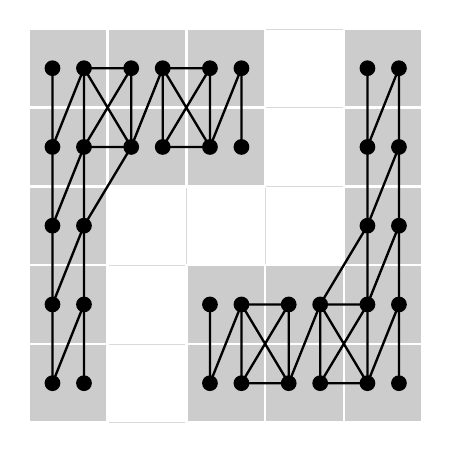
\begin{tikzpicture}
\draw[help lines, black!15] (0,0) grid (5,5);
\foreach \a in \D
    {\draw[black!0, fill=black!20, line width=0.3mm]
        \a rectangle +(1,1);
     \fill[black] foreach \b in 
        {(0.3, 0.5), (0.7, 0.5)}
        {\a++\b circle (1mm)};
    };
\draw[black, line width=0.3mm]
    foreach \a in {(0,0), (2,0), (3,0), (4,0), (0,1), (4,1), (0,2), (4,2), (0,3), (1,3), (2,3), (4,3)}
        {\a++(0.3, 0.5)--+(0, 1)
         \a++(0.3, 0.5)--+(0.4, 1)
         \a++(0.7, 0.5)--+(0, 1)}
    foreach \a in {(2,0), (3,0), (0,3), (1,3)}
        {\a++(0.7, 0.5)--+(0.6, 0)
         \a++(0.7, 0.5)--+(0.6, 1)
         \a++(0.7, 1.5)--+(0.6, 0)
         \a++(0.7, 1.5)--+(0.6, -1)}
    foreach \a in {(0,2), (3,1)}
        {\a++(0.7, 0.5)--+(0.6, 1)}
    ;
% \draw[black, line width=0.5mm] (0,0)rectangle (12,12);
\end{tikzpicture}
\end{document}